\chapter*{}
\large
$
\begin{array}{l}
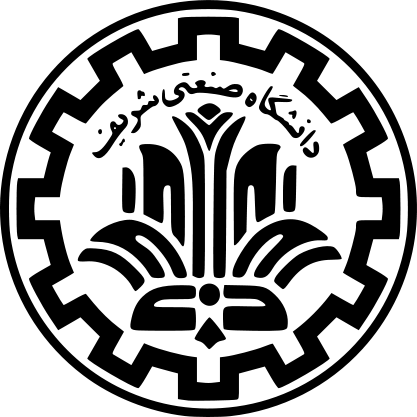
\includegraphics[width=1.6cm]{sharif.png}
\end{array}
$ \hspace{4.7cm} \textbf{اظهارنامه}
\small
\begin{center}
(اصالت متن و محتوای پایان‌نامه کارشناسی ارشد) \\
\end{center}
\vspace{0.5cm}
عنوان پایان‌نامه: 
\textbf{عنوان تز}
\\
نام استاد راهنما: 
\textbf{نام استاد راهنما}
 \hfill
نام استاد راهنمای همکار: 
\textbf{\ldots}
 \hfill
نام استاد مشاور: 
 \textbf{\ldots}
 \vspace{0.5cm}
 \\
 اینجانب \textbf{نام دانشجو} اظهار می‌دارم:
 \شروع{شمارش}
 \فقره متن و نتایج علمی ارائه‌شده در این پایان‌نامه اصیل بوده و منحصراً توسّط این‌جانب و زیر نظر استادان (راهنما، همکار و مشاور) نام‌برده شده در بالا تهیّه شده‌است.
 \فقره متن پایان‌نامه به این صورت در هیچ جای دیگری منتشر نشده‌است.
 \فقره متن و نتایج مندرج در این پایان‌نامه، حاصل تحقیقات این‌جانب به عنوان دانشجوی کارشناسی ارشد دانشگاه صنعتی شریف است.
 \فقره کلیه‌ی مطالبی که از منابع دیگر در این پایان‌نامه مورد استفاده قرار گرفته، با ذکر مرجع مشخّص شده‌است.
\پایان{شمارش}
\vspace{0.5cm}

\hspace{8cm} نام دانشجو: \textbf{نام دانشجو}

\hspace{8cm} تاریخ: \textbf{\today}

\hspace{8cm} امضاء:
\vspace{0.5cm}
\\
نتایج تحقیقات مندرج در این پایان‌نامه و دستاوردهای مادّی و معنوی ناشی از آن (شامل فرمول‌ها، توابع کتابخانه‌ای، نرم‌افزارها، سخت‌افزارها و مواردی که قابلیّت ثبت اختراع دارد) متعلّق به دانشگاه صنعتی شریف است. هیچ شخصیّت حقیقی یا حقوقی بدون کسب اجازه از دانشگاه صنعتی شریف حق فروش و ادعای مالکیّت مادّی یا معنوی بر آن یا ثبت اختراع از آن را ندارد. همچنین کلّیه‌ی حقوق مربوط به چاپ، تکثیر، نسخه‌برداری، ترجمه، اقتباس و نظائر آن در محیط‌های مختلف اعم از الکترونیکی، مجازی یا فیزیکی برای دانشگاه صنعتی شریف محفوظ است. نقل مطالب با ذکر مأخذ بلامانع است.

\vspace{0.5cm}
نام استاد راهنما: \textbf{نام استاد راهنما}
\hspace{2.9cm}
نام دانشجو: \textbf{نام دانشجو}

تاریخ: \textbf{\today}
\hspace{5.1cm}
تاریخ: \textbf{\today}

امضاء: 
\hspace{7cm}
امضاء: 

\normalsize
